\section{Network Access Layer}

\subsection{SDU/PDU}
Die Service Data Unit (SDU oder auch Payload) eines Layers ist die Protocol Data Unit (PDU) des darüberliegenden Layers. \\
PDU = Protokollinformationen-(PCI) + SDU\\
Layer 1 SDU = Layer 2 PDU
\subsection{10Base-T}

\subsubsection{Wiring}
Transmit auf Pins 1,2\\
Receive auf Pins 3,6

\subsubsection{Codierung}
Der 10Base-T Standard verwendet Manchester Codierung. Daher ist für 10Mbit Datenübertragungsraten eine echte übertragungsrate von 20Mbit erforderlich.
\subsubsection{Daten}

Bitdauer:

\begin{align}
\frac{1s}{10^{7}bits} = 100ns
\end{align}


Ausbreitung Elektromagnetischer Wellen im Kabel: 
\begin{align}
\frac{2}{3} \cdot 300\cdot 10^{6} \frac{m}{s}
\end{align}

Länge eines Bits im Kabel:
\begin{align}
100ns \cdot \frac{0.2m}{ns} = 20m
\end{align}

\subsection{100Base-TX}
\subsubsection{Wiring}
Transmit auf Pins 1,2\\
Receive auf Pins 3,6
\subsubsection{Codierung}
Der 100Base-TX Standard verwendet eines sogenanntes 4B/5B encoding (Block-Codierung). Jedem 4 bit Wort wird auf ein 5 Bit Wort abgebildet, sodass nie mehr als 3 aufeinander folgende Nullen vorhanden sind. Somit ist eine sogenannte Symbolrate von +25\%, also 125Mbps, notwendig.
Um das Übertragene Spektrum zu verkleinern, werden die Bits zusätzlich mittels MLT-3 (Multi-Level-Transition) Verfahren codiert.\\
Die Taktrückgewinnung nur mit MLT-3 codierung ist aber nicht möglich, durch die vorangegangene 4B5B Codierung jedoch schon. Zusätzlich bleiben durch die 4B5B Codierung weitere $2^5-2^4=16$ Codes übrig, die zur Synchronisation/Signalisierung verwendet werden können.


\subsubsection{Daten}
Bitdauer:
\begin{align*}
\frac{1s}{10^{8}bits} = 10ns
\end{align*}

Länge eines Bits im Kabel:
\begin{align}
10ns \cdot \frac{0.2m}{ns} = 2m
\end{align}

\subsection{MAC-Frame}
Die Minimallänge eines MAC Frames beträgt 64Byte, bedingt durch den CSMA/CD Mechanismus zur Kollisionsdetektion.
Die Maximalgrösse beträgt 1500 Bytes Payload + 12 Bytes SA/DA + 2 Bytes LEN/PT + 4Bytes Checksum = 1518 Bytes an Daten. Hinzu kommen noch 8 Bytes für Preamble und SFD.

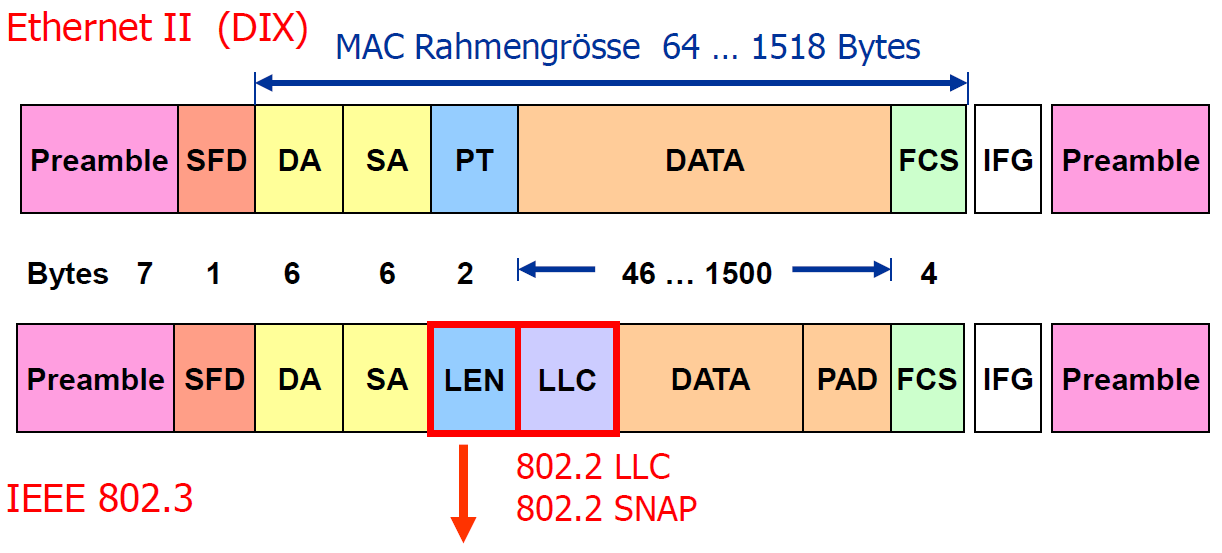
\includegraphics[scale=0.5]{media/MACFrame.png}

\subsubsection{Ethernet II}
Ethernet II (DIX) Pakete werden durch einen PT grösser als 1500 (0x05DC)gekennzeichnet. Payloadtype für IP: 0x800, für ARP: 0x806.

\subsubsection{802.3}
Ethernet 802.3 Pakete sind durch Angaben im LEN Feld kleiner als 1500 gekennzeichnet. Die Länge gibt die PDU Länge des LLC Protokolls an.

\subsection{MAC-Adressen}
das LSB im ersten Adress Byte (Most Significant Octet) der Destination Address ist das Individual/Group Bit, 0 heisst individuelle Adresse, 1 Multicast/Broadcast Adresse.\\
2. Bit ist das Universal/Local bit, 0 heisst globally administered Adresse, 1 heisst local administered Address.

\subsection{Collision}
Kollisionen könnne nur in Half-Duplex Mode Übertragungen auftreten.


\subsection{Amplitudenmodulation}
\begin{align*}
\cos (2\pi \cdot F_N) \cdot \cos (2\pi \cdot F_T)
= \frac{1}{2}(\cos (2\pi \cdot F_T - 2\pi \cdot F_N) + cos(2\pi \cdot F_T + 2\pi \cdot F_N)
\end{align*}
Somit hat sich zum einen die Regellage verschoben und es ist noch eine Kehrlage hinzugekommen: $\cos (2\pi F_T - F_N)$.
